\subsection{Скремблирование исходного сообщения}
\begin{enumerate}
	\item \textbf{Выберем алгоритм преобразования:}
	      \[
		      B_i = A_i \oplus B_{i-3} \oplus B_{i-5} \quad (i = 1, 2, \ldots, 32)
	      \]

	\item \textbf{Исходное сообщение:}
	      \[
		      \textbf{1100\ 0100\ 1110\ 0010\ 1100\ 0001\ 1100\ 0000}
	      \]

	\item \textbf{Скремблированное сообщение:}
	      \[
		      \begin{array}{ll}
			      B_1 = A_1 = 1                                                         \\
			      B_2 = A_2 = 1                                                         \\
			      B_3 = A_3 = 0                                                         \\
			      B_4 = A_4 \oplus B_1 = 0 \oplus 1 = 1                                 \\
			      B_5 = A_5 \oplus B_2 = 0 \oplus 1 = 1                                 \\
			      B_6 = A_6 \oplus B_3 \oplus B_1 = 1 \oplus 0 \oplus 1 = 0             \\
			      B_7 = A_7 \oplus B_4 \oplus B_2 = 0 \oplus 1 \oplus 1 = 0             \\
			      B_8 = A_8 \oplus B_5 \oplus B_3 = 0 \oplus 1 \oplus 0 = 1             \\
			      B_9 = A_9 \oplus B_6 \oplus B_4 = 1 \oplus 0 \oplus 1 = 0             \\
			      B_{10} = A_{10} \oplus B_7 \oplus B_5 = 1 \oplus 0 \oplus 1 = 0       \\
			      B_{11} = A_{11} \oplus B_8 \oplus B_6 = 1 \oplus 1 \oplus 0 = 0       \\
			      B_{12} = A_{12} \oplus B_9 \oplus B_7 = 0 \oplus 0 \oplus 0 = 0       \\
			      B_{13} = A_{13} \oplus B_{10} \oplus B_8 = 0 \oplus 0 \oplus 1 = 1    \\
			      B_{14} = A_{14} \oplus B_{11} \oplus B_9 = 0 \oplus 0 \oplus 0 = 0    \\
			      B_{15} = A_{15} \oplus B_{12} \oplus B_{10} = 1 \oplus 0 \oplus 0 = 1 \\
			      B_{16} = A_{16} \oplus B_{13} \oplus B_{11} = 0 \oplus 1 \oplus 0 = 1 \\
			      B_{17} = A_{17} \oplus B_{14} \oplus B_{12} = 1 \oplus 0 \oplus 0 = 1 \\
			      B_{18} = A_{18} \oplus B_{15} \oplus B_{13} = 1 \oplus 1 \oplus 1 = 1 \\
			      B_{19} = A_{19} \oplus B_{16} \oplus B_{14} = 0 \oplus 1 \oplus 0 = 1 \\
			      B_{20} = A_{20} \oplus B_{17} \oplus B_{15} = 0 \oplus 1 \oplus 1 = 0 \\
			      B_{21} = A_{21} \oplus B_{18} \oplus B_{16} = 0 \oplus 1 \oplus 1 = 0 \\
			      B_{22} = A_{22} \oplus B_{19} \oplus B_{17} = 0 \oplus 1 \oplus 1 = 0 \\
			      B_{23} = A_{23} \oplus B_{20} \oplus B_{18} = 0 \oplus 0 \oplus 1 = 1 \\
			      B_{24} = A_{24} \oplus B_{21} \oplus B_{19} = 1 \oplus 0 \oplus 1 = 0 \\
			      B_{25} = A_{25} \oplus B_{22} \oplus B_{20} = 1 \oplus 0 \oplus 0 = 1 \\
			      B_{26} = A_{26} \oplus B_{23} \oplus B_{21} = 1 \oplus 1 \oplus 0 = 0 \\
			      B_{27} = A_{27} \oplus B_{24} \oplus B_{22} = 0 \oplus 0 \oplus 0 = 0 \\
			      B_{28} = A_{28} \oplus B_{25} \oplus B_{23} = 0 \oplus 1 \oplus 1 = 0 \\
			      B_{29} = A_{29} \oplus B_{26} \oplus B_{24} = 0 \oplus 0 \oplus 0 = 0 \\
			      B_{30} = A_{30} \oplus B_{27} \oplus B_{25} = 0 \oplus 0 \oplus 1 = 1 \\
			      B_{31} = A_{31} \oplus B_{28} \oplus B_{26} = 0 \oplus 0 \oplus 0 = 0 \\
			      B_{32} = A_{32} \oplus B_{29} \oplus B_{27} = 0 \oplus 0 \oplus 0 = 0 \\
		      \end{array}
	      \]

	\item Получили новое сообщение, в котором всё равно присутствует достаточно длинная последовательность из 4х нулей, но главное избавились от последовательностей из 6 и из 5 нулей в исходном сообщении, что существенно улучшит синхронизацию.

	\item \textbf{Результат скремблирования: (в двоичном виде)}
	      \[
		      \textbf{1101\ 1001\ 0000\ 1011\ 1110\ 0001\ 1000\ 0100}
	      \]

	\item \textbf{Результат скремблирования (в шестнадцатеричном виде):}
	      \[
		      \textbf{D9 0B E1 84}
	      \]
\end{enumerate}

По аналогичным причинам, что я описал в конце этапа избыточного кодирования, применю скремблированное сообщение для кодирования NRZI.
\subsection{Применим для кодирования NRZI}
\begin{figure}[H]
	\centering
	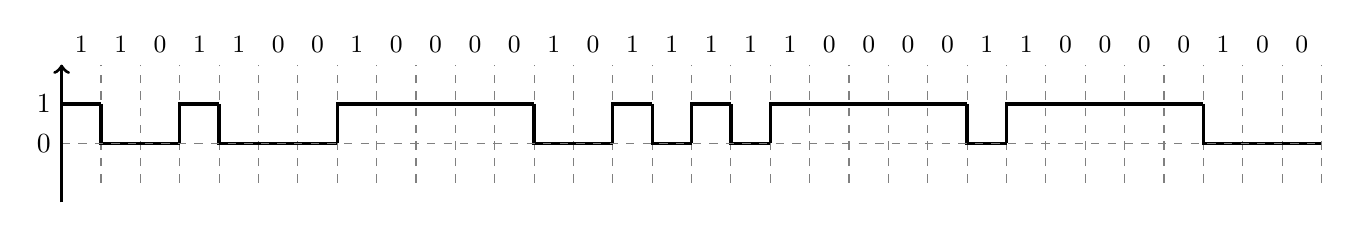
\begin{tikzpicture}[scale=0.5, very thick]
		\def\bits{1,1,0,1,1,0,0,1,0,0,0,0,1,0,1,1,1,1,1,0,0,0,0,1,1,0,0,0,0,1,0,0}

		\gdef\y{0}
		\foreach \b [count=\x from 0] in \bits {
			\draw[dashed, gray, thin] (\x+1,-1) -- (\x+1,2);
			\node at (\x+0.5, 2.5) {\small \b};
			\ifnum\b=1
				\ifnum\y=1
					\draw (\x,1) -- (\x,0) -- (\x+1,0);
					\xdef\y{0}
				\else
					\draw (\x,0) -- (\x,1) -- (\x+1,1);
					\xdef\y{1}
				\fi
			\else
				\draw (\x,\y) -- (\x+1,\y);
			\fi
		}

		\draw[dashed, gray, thin] (0,0) -- (32,0);
		\draw[->] (0,-1.5) -- (0,2);

		\node[left] at (0,0) {0};
		\node[left] at (0,1) {1};
	\end{tikzpicture}
	\caption{NRZI-кодирование избыточного сообщения}
\end{figure}

\begin{figure}[H]
	\centering
	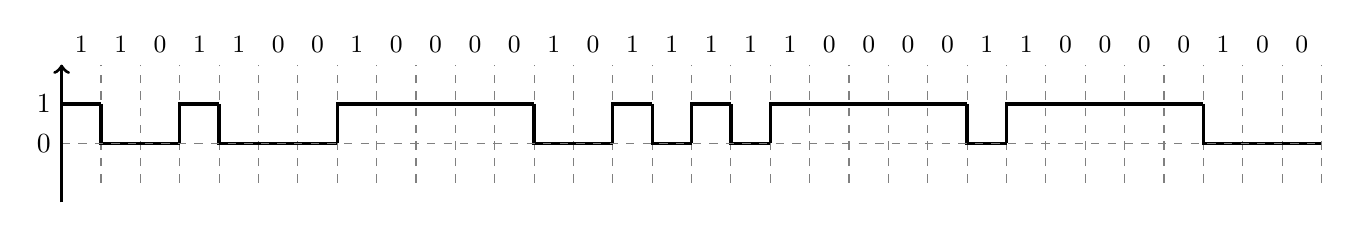
\begin{tikzpicture}[scale=0.5, very thick]
		\def\bits{1,1,0,1,1,0,0,1,0,0,0,0,1,0,1,1,1,1,1,0,0,0,0,1,1,0,0,0,0,1,0,0}

		\gdef\y{0}
		\foreach \b [count=\x from 0] in \bits {
			\draw[dashed, gray, thin] (\x+1,-1) -- (\x+1,2);
			\node at (\x+0.5, 2.5) {\small \b};
			\ifnum\b=1
				\ifnum\y=1
					\draw (\x,1) -- (\x,0) -- (\x+1,0);
					\xdef\y{0}
				\else
					\draw (\x,0) -- (\x,1) -- (\x+1,1);
					\xdef\y{1}
				\fi
			\else
				\draw (\x,\y) -- (\x+1,\y);
			\fi
		}

		\draw[dashed, gray, thin] (0,0) -- (32,0);
		\draw[->] (0,-1.5) -- (0,2);

		\node[left] at (0,0) {0};
		\node[left] at (0,1) {1};
	\end{tikzpicture}
	\caption{NRZI-кодирование избыточного сообщения}
\end{figure}

